\section{Presentazioni}
  \texttt{\textbackslash{}documentclass[aspectratio=169]\{beamer\} \% prima riga}
  \texttt{\\\dots\\
  \textbackslash{}begin\{frame\} \%dentro il document
\\
  ~~\textbackslash{}frametitle\{Titolo\}~~~~~~~~~~~~~
\\
  ~~\textbackslash{}framesubtitle\{Sottotitolo\}~~~~~
\\
  \textbackslash{}end\{frame\}
~~~~~~~~~~~~~~~~~~~~~~~\\~}
  \subsection{Comandi noti}
  Titolo: \texttt{\textbackslash{}maketitle}\\~\\
  \texttt{\textbackslash{}section, \textbackslash{}subsection}\\~\\
  Formattazione testo, immagini, note a piè di pagina, bibliografia, \dots

  \subsection{Indice}
  \texttt{~\\
  \textbackslash{}begin\{frame\}~~~~~~~~~~~\\
  ~~\textbackslash{}frametitle\{Contenuti\}\\
  ~~\textbackslash{}tableofcontents~~~~~~~~\\
  \textbackslash{}end\{frame\}~~~~~~~~~~~~~\\~
}
\subsection{Animazioni}
  \texttt{Questa è \textbackslash{}pause una prova}
\subsection{Temi e colori}
  \begin{tabular}{ll}
    \texttt{\textbackslash{}usetheme\{Warsaw\}}& Esempi di tutte le combinazioni tema-colore:\\
    \texttt{\textbackslash{}usecolortheme\{seahorse\}} & \url{https://hartwork.org/beamer-theme-matrix/}
  \end{tabular}
  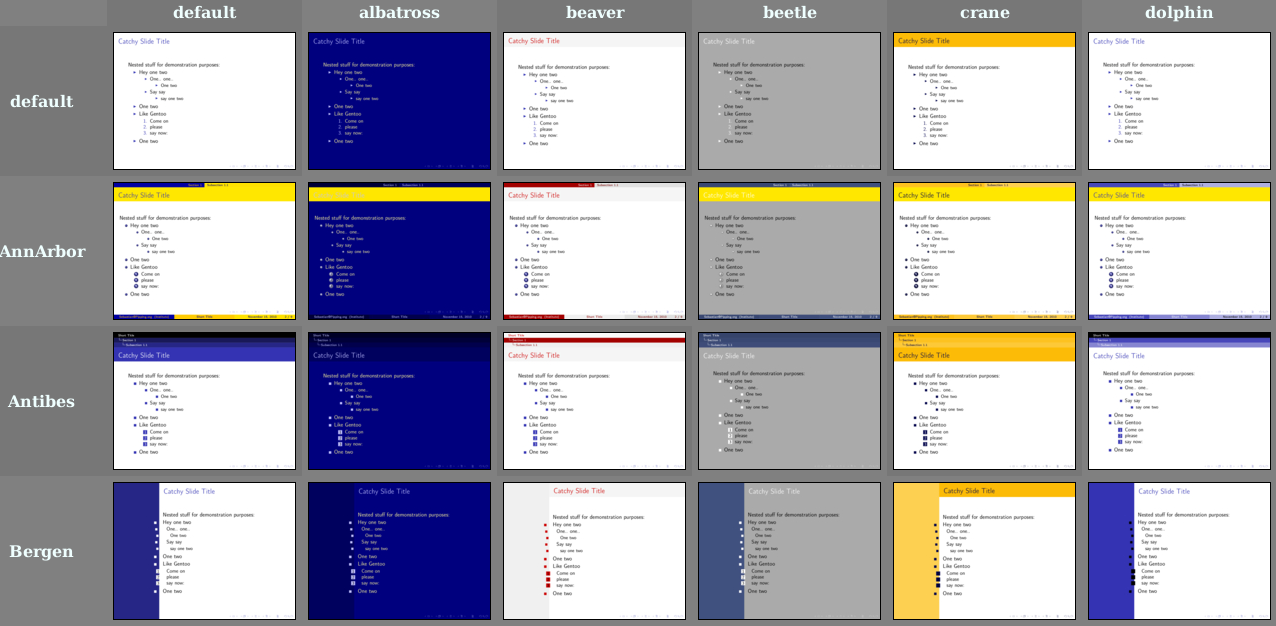
\includegraphics[width=\textwidth]{img/beamer}

